
\section{Software und \emph{Cloud}}
Dieser Abschnitt behandelt die verwendete bzw. implementierte Software und die verwendeten Dienste für die Applikation \emph{RPISec}.

\subsection{\emph{Microservices}}
Dieser Abschnitt behandelt die auf dem \emph{Raspberry PI} gehosteten Services. Die Services wurden mit \emph{Spring Boot} als \emph{Microservices} implementiert, was möglich war, da Oracle eine ARM Implementierung der Java-JDK bereitstellt und die \emph{Microservices} schlank implementiert wurden, sodass die zur Verfügung stehenden Ressourcen ausreichen, um diese Services auf einen \emph{Raspberry PI} zu betreiben.
\newline
\newline
Es wurden die beiden \emph{Microservices Auth-Service} für die Benutzerverwaltung und OAuth2 Authentifizierung und \emph{App-Service} für die Interaktion mit der Sensorapplikation und der Interaktion mit dem \emph{Cloud} Dienst implementiert, wobei der \emph{Microservice Auth-service} im Zuge des Projekts für die Lehrveranstaltung \emph{Service Engineering} implementiert wurde. Es hätte auch ausgereicht die Benutzerverwaltung in den \emph{Microservice App-Service} zu verpacken, obwohl dann der \emph{Microservice} für zwei Aspekte verantwortlich gewesen wäre, was im Widerspruch zu einem \emph{Microservice} steht, der nur für einen Aspekt verantwortlich sein soll. 
\newline
\newline
Der \emph{Microservice App-Service} interagiert nicht direkt mit der Sensorik, sondern bindet die Sensorapplikation beschrieben in Abschnitt \ref{sec:sensor-application} ein und ist für dessen Lebenszyklus verantwortlich. Nachdem Start der Sensorapplikation wird ein \emph{Listener} registriert, der auf Statusänderungen des Bewegungssensor reagiert und diesen Sicherheitsverstoß wie in Abbildung \ref{fig:image-sequence-incident} behandelt.

\subsection{Sensor Applikation}
\label{sec:sensor-application}
Bei den Komponenten der Sensor-Anwendung handelt es sich, wie in \autoref{sec:raspberrypi} erwähnt, um die beiden Bauteile:

\begin{itemize}
	\item \emph{AZDeliveryCamRasp Kamera}
	\item \emph{HC-SR501 Bewegungssensor}
\end{itemize}
\ \newline
Die Ansteuerung der Pins erfolgt über die \emph{Pi4J\footnote{\url{http://pi4j.com/}}}-Bibliotheken die wiederum die \emph{WiringPi\footnote{\url{http://wiringpi.com/}}}-Bibliothek nutzt, welche die eigentliche Ansteuerung der Pins erledigt.

\subsubsection{Pi4J}
Pi4J ist eine Bibliothek  für Java, die den vollen Zugriff auf die Ressourcen des \emph{Raspberry PI} ermöglicht. Mit Pi4J ist es möglich Anwendungen für \emph{Raspberry PI} zu schreiben, die nur Java benötigen. Damit können praktisch alle Bibliotheken eingesetzt werden, die für Java verfügbar sind. Einschränkungen gibt es nur bei den Ressourcen des \emph{Raspberry PI}.

\subsubsection{WiringPi}
\emph{WiringPi} ist eine Bibliothek, um die \emph{GPIO} Ein-und Ausgänge am \emph{Raspberry Pi} zu schalten. Das Ziel dieser Bibliothek ist es, eine einzige gemeinsame Plattform und Programmierschnistelle für den Zugriff auf die \emph{GPIOs} des \emph{Rapsberry Pi} für verschiedene Programmiersprachen zur Verfügung zu stellen. Im Kern ist \emph{WiringPi} eine C-Bibliothek, aber sie steht auch in Ruby und Python zur Verfügung.
\newpage

\begin{code}
	\caption{IRSensor\_HCSR501.java}
	\javaFile{\srcDir/gpio-controller.java}
	\label{src:gpio-controller}
\end{code}

\subsection{Mobiler \emph{Client}}
Beim \emph{RPISec Client} handelt es sich um eine native \emph{Android App}. Diese kommuniziert über REST-Schnittstellen mit einem \emph{Auth-Service} sowie mit \emph{Firebase}-Diensten von Google. Die für diese App verwendeten \emph{Firebase}-Dienste sind \emph{Firebase-Messaging} und \emph{Firebase-RealTimeDatabase}.\\

\subsubsection{Login}
Die Startseite der App besteht nur aus einem Login-Fenster (\autoref{fig:android_login}). Der Login erfolgt in drei Schritten.

\begin{enumerate}
	\item RPISec Login
	\newline
	\newline
	Die App generiert einen UUID-Wert \emph{(Universally Unique Identifier)} als Identifikator für das Gerät. Zusammen mit dem eingegebenen Benutzernamen, Passwort und der UUID wird eine Anfrage für einen \emph{Firebase}-Token an den \emph{Auth-Service} gestellt. Sind die Zugangsdaten korrekt, wird für diese UUID ein Token, sowie \emph{Client-Id} und \emph{Client-Secret} erzeugt und als Antwort an die \emph{App} übertragen. Der \emph{Firebase}-Token wird für die Authentifizierung bei den verbunden Diensten benutzt.
	\newpage
	
	\begin{code}
		\caption{ClientLoginOAuthTask.java}
		\javaFile{\srcDir/ClientLoginOAuthTask.java}
		\label{src:ClientLoginOAuthTask}
	\end{code}
		
	\item  \emph{Firebase} Login
	\newline
	\newline
	Im zweiten Schritt wird ein Token für \emph{Firebase-Messaging} registriert. Dies erfolgt wiederum mit dem Benutzernamen und Passwort. Nach der Registrierung kann die \emph{App} Nachrichten über den \emph{Firebase-Messageing} Dienst empfangen.\\
	
	\begin{code}
		\caption{RegisterFCMTask.java}
		\javaFile{\srcDir/RegisterFCMTask.java}
		\label{src:RegisterFCMTask}
	\end{code}

	\item \emph{Firebase}-Token Registrierung 
	\newline
	\newline
	Am Schluss wird der \emph{Firebase}-Token am \emph{Auth-Service} registriert.
 \end{enumerate}
\ \newpage

\begin{figure}
	\centering
	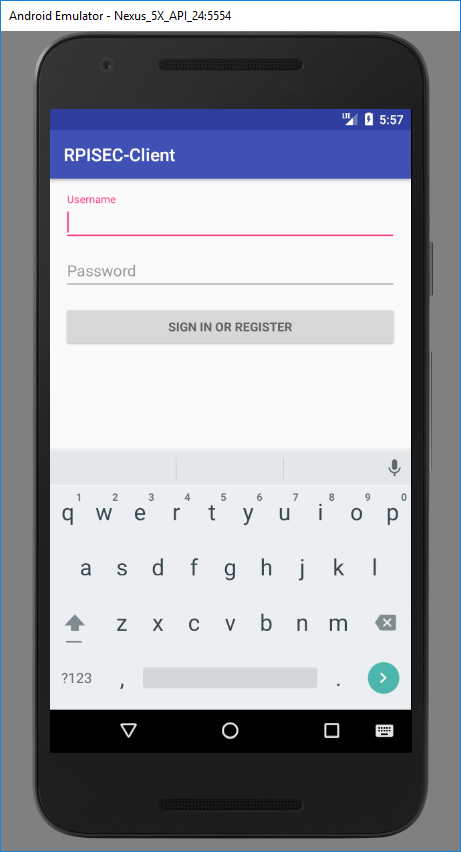
\includegraphics[scale=0.6]{\imageDir/android_login.png}
	\caption{Pin-Schema}
	\label{fig:android_login}
\end{figure}

Nach einem erfolgreichen Login wird automatisch die Detailansicht (siehe \autoref{fig:android_image_overview_m}) gestartet.
\newpage

\subsubsection{Detailansicht}
Bei der Detailansicht handelt es sich um eine Übersicht aller Bilder, chronologisch geordnet nach Aufnahmedatum, in einem Raster. Bei den angezeigten Bildern handelt es sich nur um \emph{Thumbnails}. Die richtigen Bilder werden beim Auswählen eines Bildes angezeigt, ähnlich dem \emph{Fotoviewer} in Android.
\newline
\newline
Die Detailansicht wird beim Eintreffen eines neuen Bildes aktualisiert. Sollte die Detailansicht nicht die aktive Anwendung sein, wird in der Infoleiste eine Notifikation angezeigt und ein Ton abgespielt. Durch tippen auf die Notifikation wird die Anwendung wieder in den Vordergrund geholt.
\newline
\newline
Mittels Swipe-Down-Geste kann die Ansicht aktualisiert werden.
\begin{figure}[h]
	\centering
	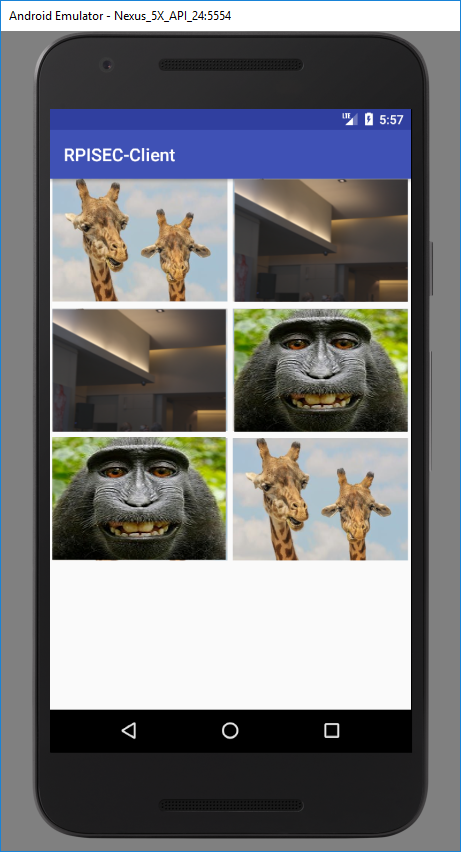
\includegraphics[scale=0.7]{\imageDir/android_image_overview_m.png}
	\caption{Pin-Schema}
	\label{fig:android_image_overview_m}
\end{figure}

\subsubsection{Datenabfrage}
Bei jedem \emph{Incident} der von der Server-Anwendung über Firebase-Messaging an die App gesendet wird, werden der Titel, eine Nachricht und die Id des aufgenommenen Bildes übertragen. Mit dieser Id kann das eigentliche Bild aus der Firebase-RealTimeDatabase abgerufen werden.\\

\begin{code}
	\caption{FirebaseMessaging.java}
	\javaFile{\srcDir/FirebaseMessaging.java}
	\label{src:FirebaseMessaging}
\end{code}

\subsection{Datenbank}
Dieser Abschnitt behandelt die verwendete Datenbank für die \emph{Microservices}. Im Entwicklungsbetrieb auf einen Entwicklerrechner wird die Datenbank H2 und im produktiven Betrieb auf einen \emph{Raspberry PI} die Datenbank PostgreSQL verwendet. Die Datenbank PostgreSQL konnte am \emph{Raspberry PI} verwendet werden, da PostgreSQL die ARM Architektur unterstützt und sich auch mit geringen Ressourcenaufwand betreiben lässt.

\subsection{\emph{Firebase}}
Dieser Abschnitt behandelt den verwendeten \emph{Cloud} Dienst \emph{Firebase}. \emph{Firebase} ist ein \emph{Cloud} Dienst von \emph{Google}, der einen \emph{Messaging} Dienst sowie eine Onlinedatenbank (JSON-Datenbank) bereitstellt. Bis zu einer gewissen Anzahl von \emph{Requests} ist dieser Dienst kostenlos zu verwenden.  
\newline
\newline
Für \emph{Firebase} gibt es eine Java Implementierung das sogenannte \emph{firebase-admin-sdk}, das eine API zum Interagieren mit der JSON-Datenbank und eine API zum Erstellen von Authentifizierungstoken für die \emph{Client}-Authentifizierung auf \emph{Firebase} zur Verfügung stellt. In der Java Implementierung wird zurzeit keine API für die Interaktion mit dem \emph{Messaging} Dienst zur Verfügung gestellt, was aber kein Problem darstellt, da es sich hierbei um eine einfache Anfrage an eine \emph{REST-API} handelt, die mit Spring \emph{RestTemplate} realisiert wurde.
\newline
\newline
Für die Interaktion mit \emph{Firebase} über \emph{Android} wird ebenfalls eine Java Implementierung bereitgestellt. Diese Implementierung enthält auch eine \emph{API} für den \emph{Messaging} Dienst von \emph{Firebase}.
\newline
\newline
\begin{figure}[h]
	\centering
	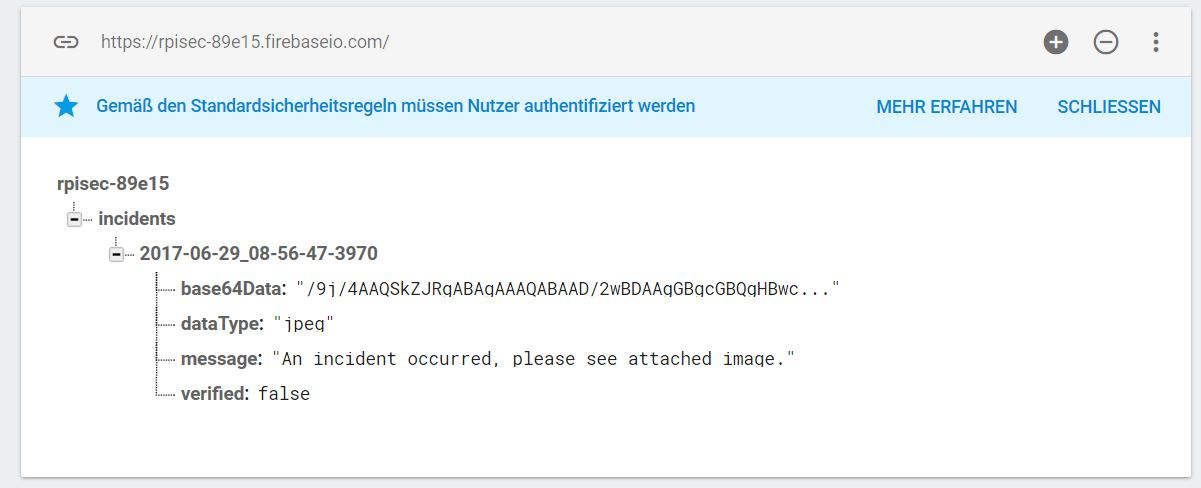
\includegraphics[scale=0.5]{\imageDir/firebase-database-entry.JPG}
	\caption{Eintrag in der \emph{Firebase} Onlinedatenbank}
	\label{fig:firabse-database}
\end{figure}
